\documentclass{article}
\usepackage{graphicx} % Required for inserting images
\usepackage{amsthm,amsmath,amssymb}
\usepackage[UTF8]{ctex}
\usepackage[tc]{titlepic}
\usepackage{titlesec}
\usepackage{cite}
\usepackage{fancyhdr}
\usepackage{booktabs}
\usepackage{subfigure}
\usepackage{float}
\usepackage[textwidth=14.5cm]{geometry}
\usepackage[section]{placeins}
\usepackage{makeidx}
\usepackage{mathrsfs}
\usepackage{color}
\usepackage{ulem}
\usepackage{enumitem}
\geometry{a4paper,scale=0.8,left=2cm,right=2cm}
\pagestyle{fancy}
\usepackage{microtype}
\usepackage{hyperref}
\usepackage{tcolorbox}
\usepackage{listings}

\lstset{
    language=Python, % 指定编程语言,如 Python、Java、C++ 等
    basicstyle=\footnotesize\ttfamily, % 调小字体大小
    keywordstyle=\color{blue}, % 关键字颜色
    commentstyle=\color{green!50!black}, % 注释颜色
    stringstyle=\color{red}, % 字符串颜色
    numbers=left, % 行号显示位置,left 表示在左侧显示
    numberstyle=\tiny\color{gray}, % 行号字体样式
    stepnumber=1, % 行号递增步长
    numbersep=5pt, % 行号与代码之间的间距
    backgroundcolor=\color{gray!10}, % 代码块背景颜色
    showspaces=false, % 不显示空格
    showstringspaces=false, % 不显示字符串中的空格
    showtabs=false, % 不显示制表符
    tabsize=2 % 制表符宽度
}


% 定义一个自定义命令,参数 #1 为中间的文字
\newcommand{\sectiondivider}[1]{%
  \vspace{1em} % 上下间距,可根据需要调整
  \begin{center}
    \noindent
    \makebox[0.3\linewidth]{\hrulefill}%
    \hspace{0.5em}% 左右间距
    {\Large\textbf{#1}}%
    \hspace{0.5em}%
    \makebox[0.3\linewidth]{\hrulefill}%
  \end{center}
  \vspace{3em}
}


\lhead{第 1 次作业\\\today}
\chead{中国科学技术大学\\	DS4001 人工智能原理与技术}

\rhead{Homework 1\\ {\CTEXoptions[today=old]\today}}
\newcommand{\upcite}[1]{\textsuperscript{\cite{#1}}}

\titleformat*{\section}{\bfseries\Large}
\titleformat*{\subsection}{\bfseries\large}

\title{\bfseries DS4001-25SP-HW1:搜索}
\author{刘芮希\quad PB22010402}

\begin{document}
%\begin{sloopypar}
\maketitle
% \clearpage

\setcounter{section}{-1}
\section{代码理解[20\%]}

\begin{enumerate}[label=(\alph*)]
    \item \textbf{[截图]} %0a
    \begin{figure}[h]
    	\centering
    	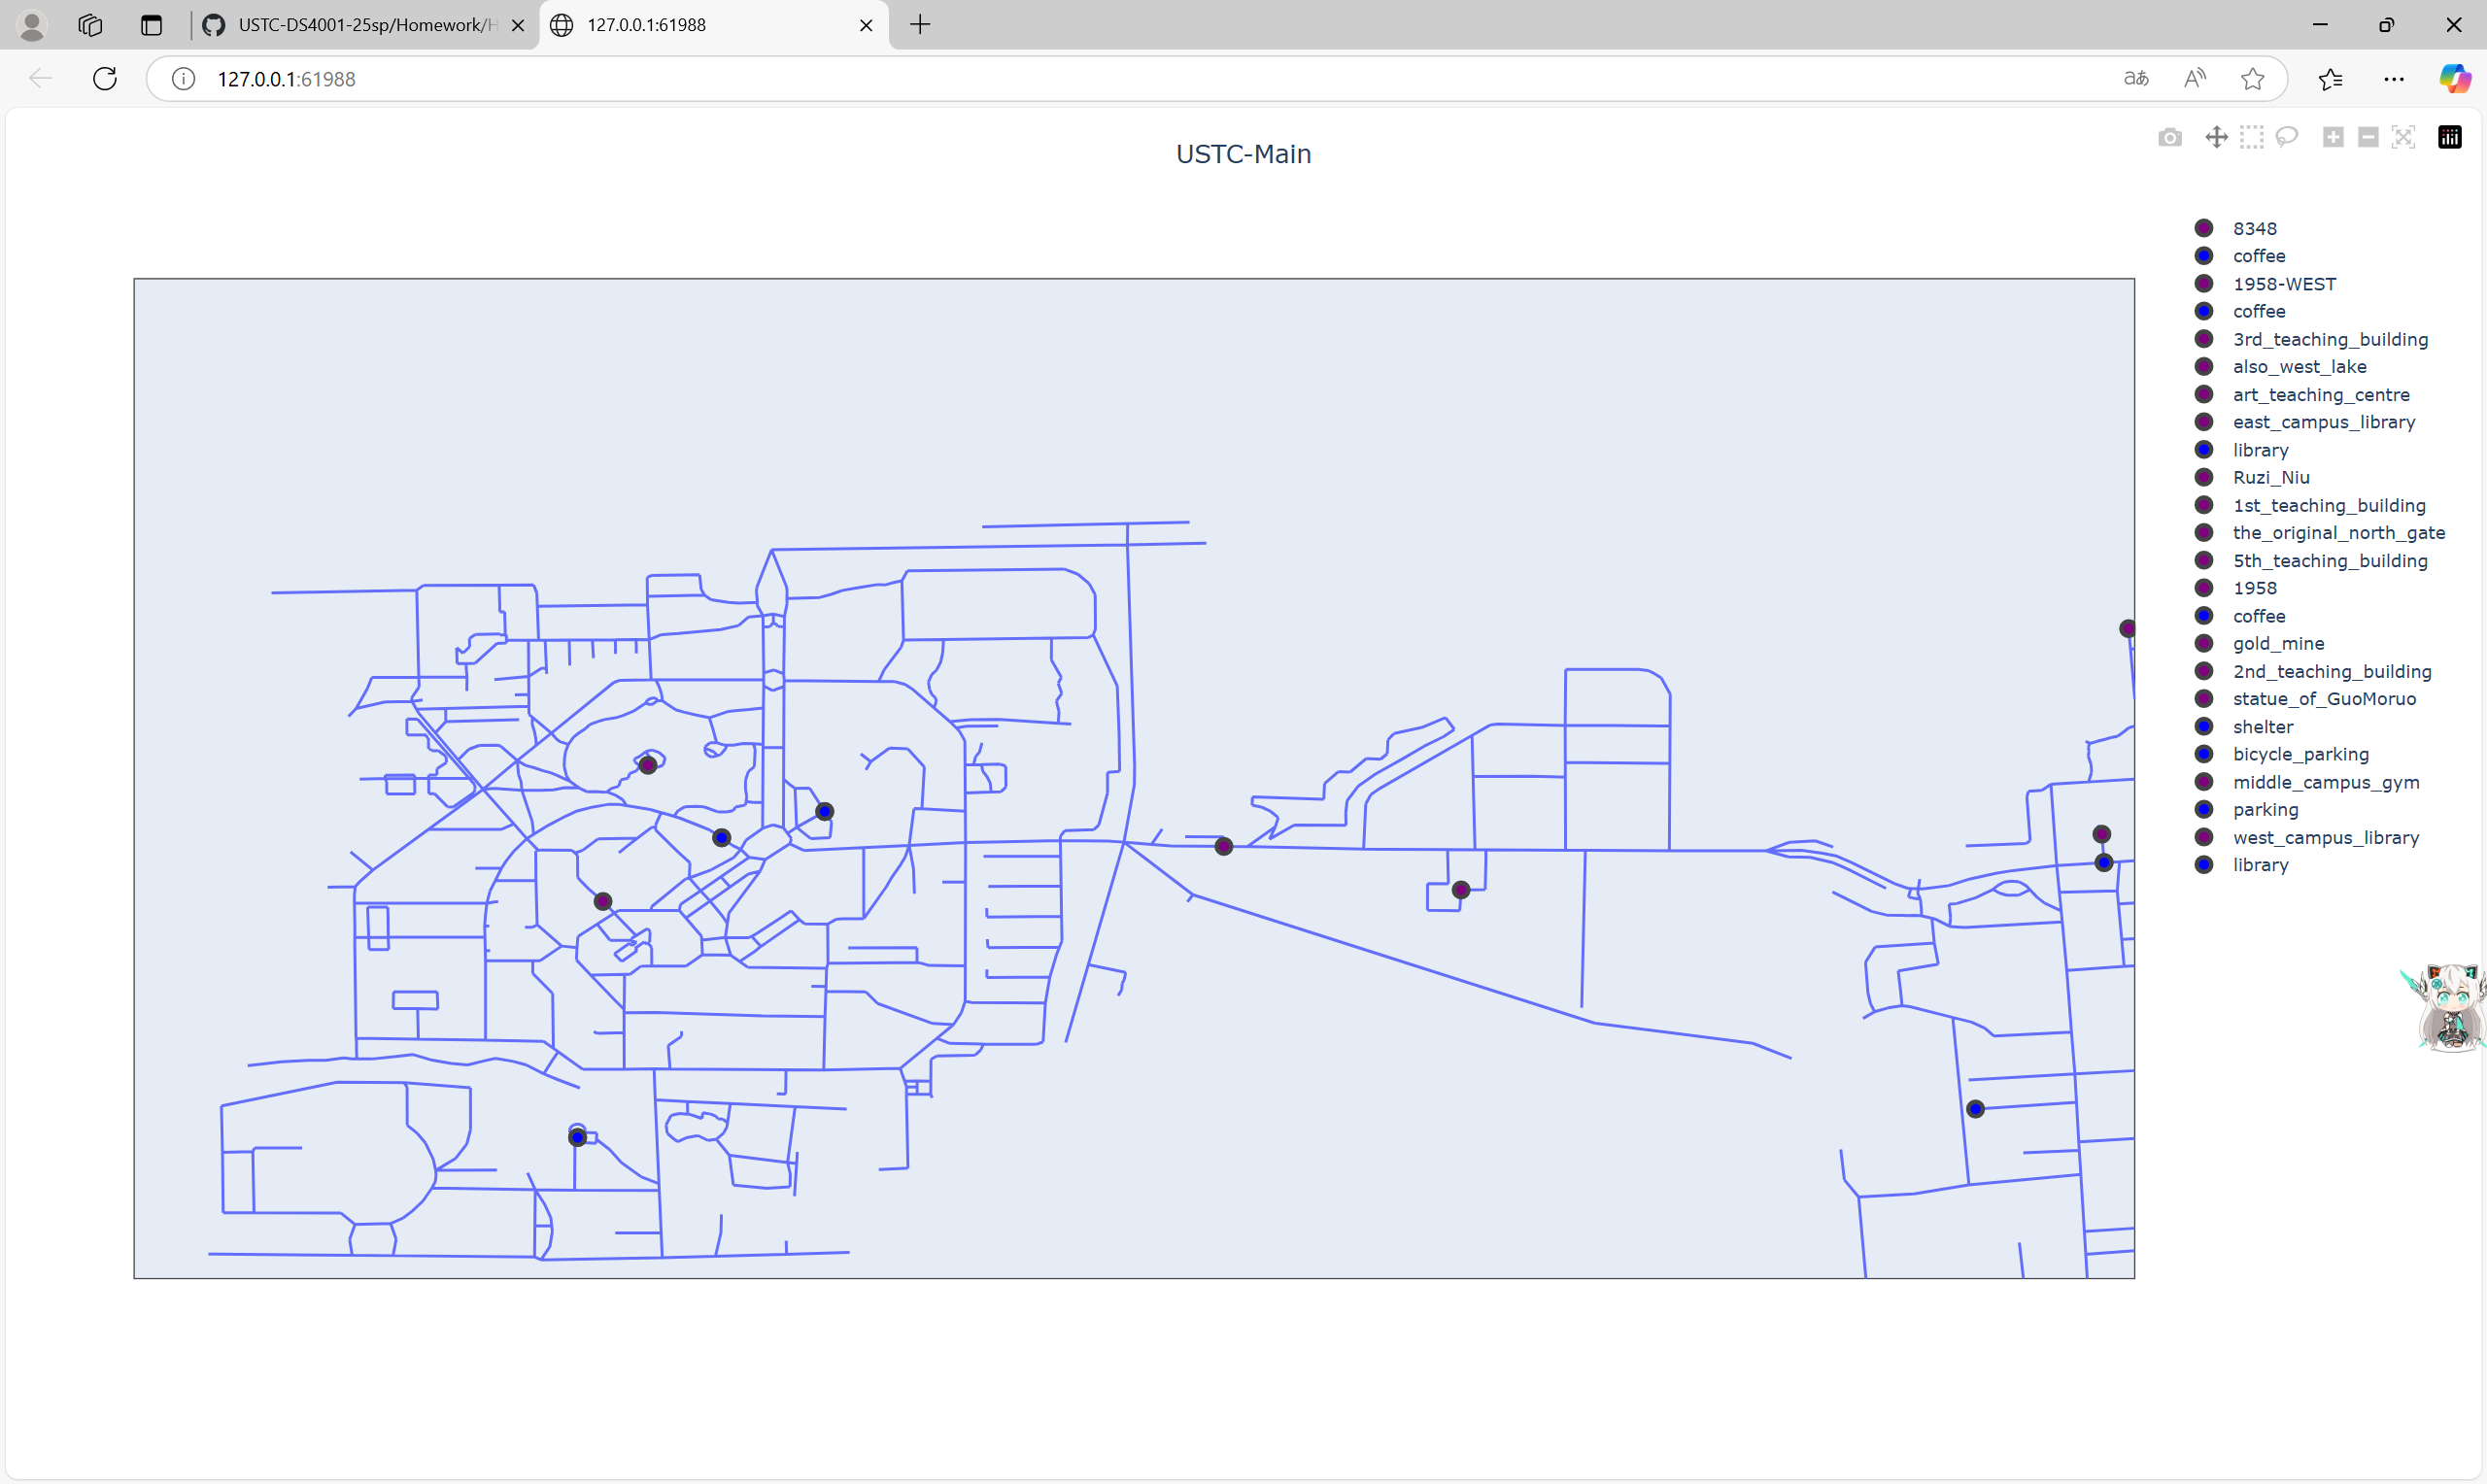
\includegraphics[width=0.8\textwidth]{visualization_result.png}
    	\caption{visualization.py结果}
    \end{figure}
\end{enumerate}


\subsection{整体结构分析[6\%]}

\begin{enumerate}[label=(\alph*), start=2]
    \item \textbf{[配对]} %0b
    \begin{itemize}
        \item \texttt{(1):}C
        \item \texttt{(2):}E
        \item \texttt{(3):}F
        \item \texttt{(4):}D
        \item \texttt{(5):}A
        \item \texttt{(6):}B
        \item \texttt{(7):}G
    \end{itemize}
\end{enumerate}

\subsection{详细代码阅读[10\%=2\%*5]}

\begin{enumerate}[label=(\alph*), start=3]
    \item \textbf{[多选]} ABE %0c
    \vspace{10pt}

    \item \textbf{[单选]} B %0d
    \vspace{10pt}

    \item \textbf{[多选]} ABC %0e
    \vspace{10pt}
\end{enumerate}

\begin{enumerate}[label=(\alph*), start=6]
    \item \textbf{[多选]} ABCDE %0f
    \vspace{10pt}

    \item  \textbf{[简答]} %0g
    \begin{figure}[h]
    	\centering
    	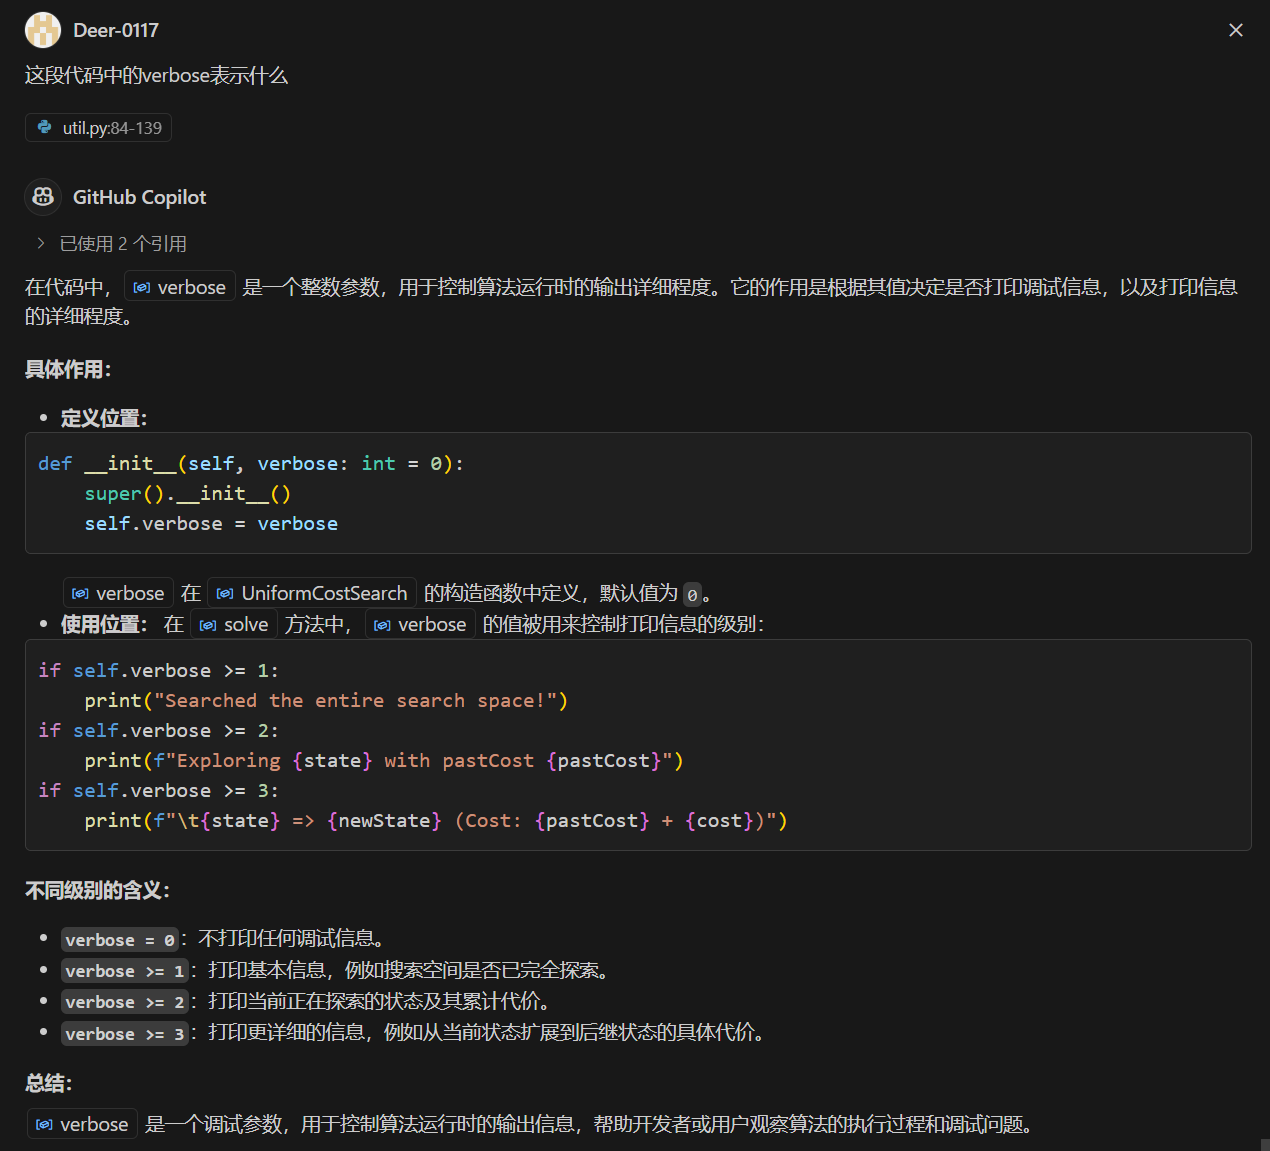
\includegraphics[width=0.8\textwidth]{verbose.png}
    	\caption{verbose表示}
    \end{figure}
\end{enumerate}

\section{问题 1:查找最短路径[29\%]}

\subsection{建模[10\%=6\%+4\%]}

\begin{enumerate}[label=(\alph*), start=1]
    \item \textbf{[代码]} %1a
    \begin{lstlisting}[language=Python]
    class ShortestPathProblem(SearchProblem):
    	def __init__(self, startLocation: str, endTag: str, cityMap: CityMap):
    		self.startLocation = startLocation
    		self.endTag = endTag
    		self.cityMap = cityMap
    
    	def startState(self) -> State:
    		return State(location=self.startLocation, memory=None)
    
    	def isEnd(self, state: State) -> bool:
    		return self.endTag in self.cityMap.tags.get(state.location, [])
    
    	def successorsAndCosts(self, state: State) -> List[Tuple[str, State, float]]:
    		successors = []
    		for neighbor, cost in self.cityMap.distances.get(state.location, {}).items():
    			action = neighbor
    			newState = State(location=neighbor, memory=None)
    			successors.append((action, newState, cost))
    		return successors
    \end{lstlisting}

    \item \textbf{[代码]} \textbf{[截图]} %1b
    建立从西区图书馆到中区东门最短路问题的实例
    \begin{lstlisting}[language=Python]
    def getUSTCShortestPathProblem() -> ShortestPathProblem:
    	cityMap = createUSTCMap()
    	startLocation = "10588133363"
    	endTag = "landmark=west_campus_library"
    	return ShortestPathProblem(startLocation, endTag, cityMap)
    \end{lstlisting}
    \begin{figure}[h]
    	\centering
    	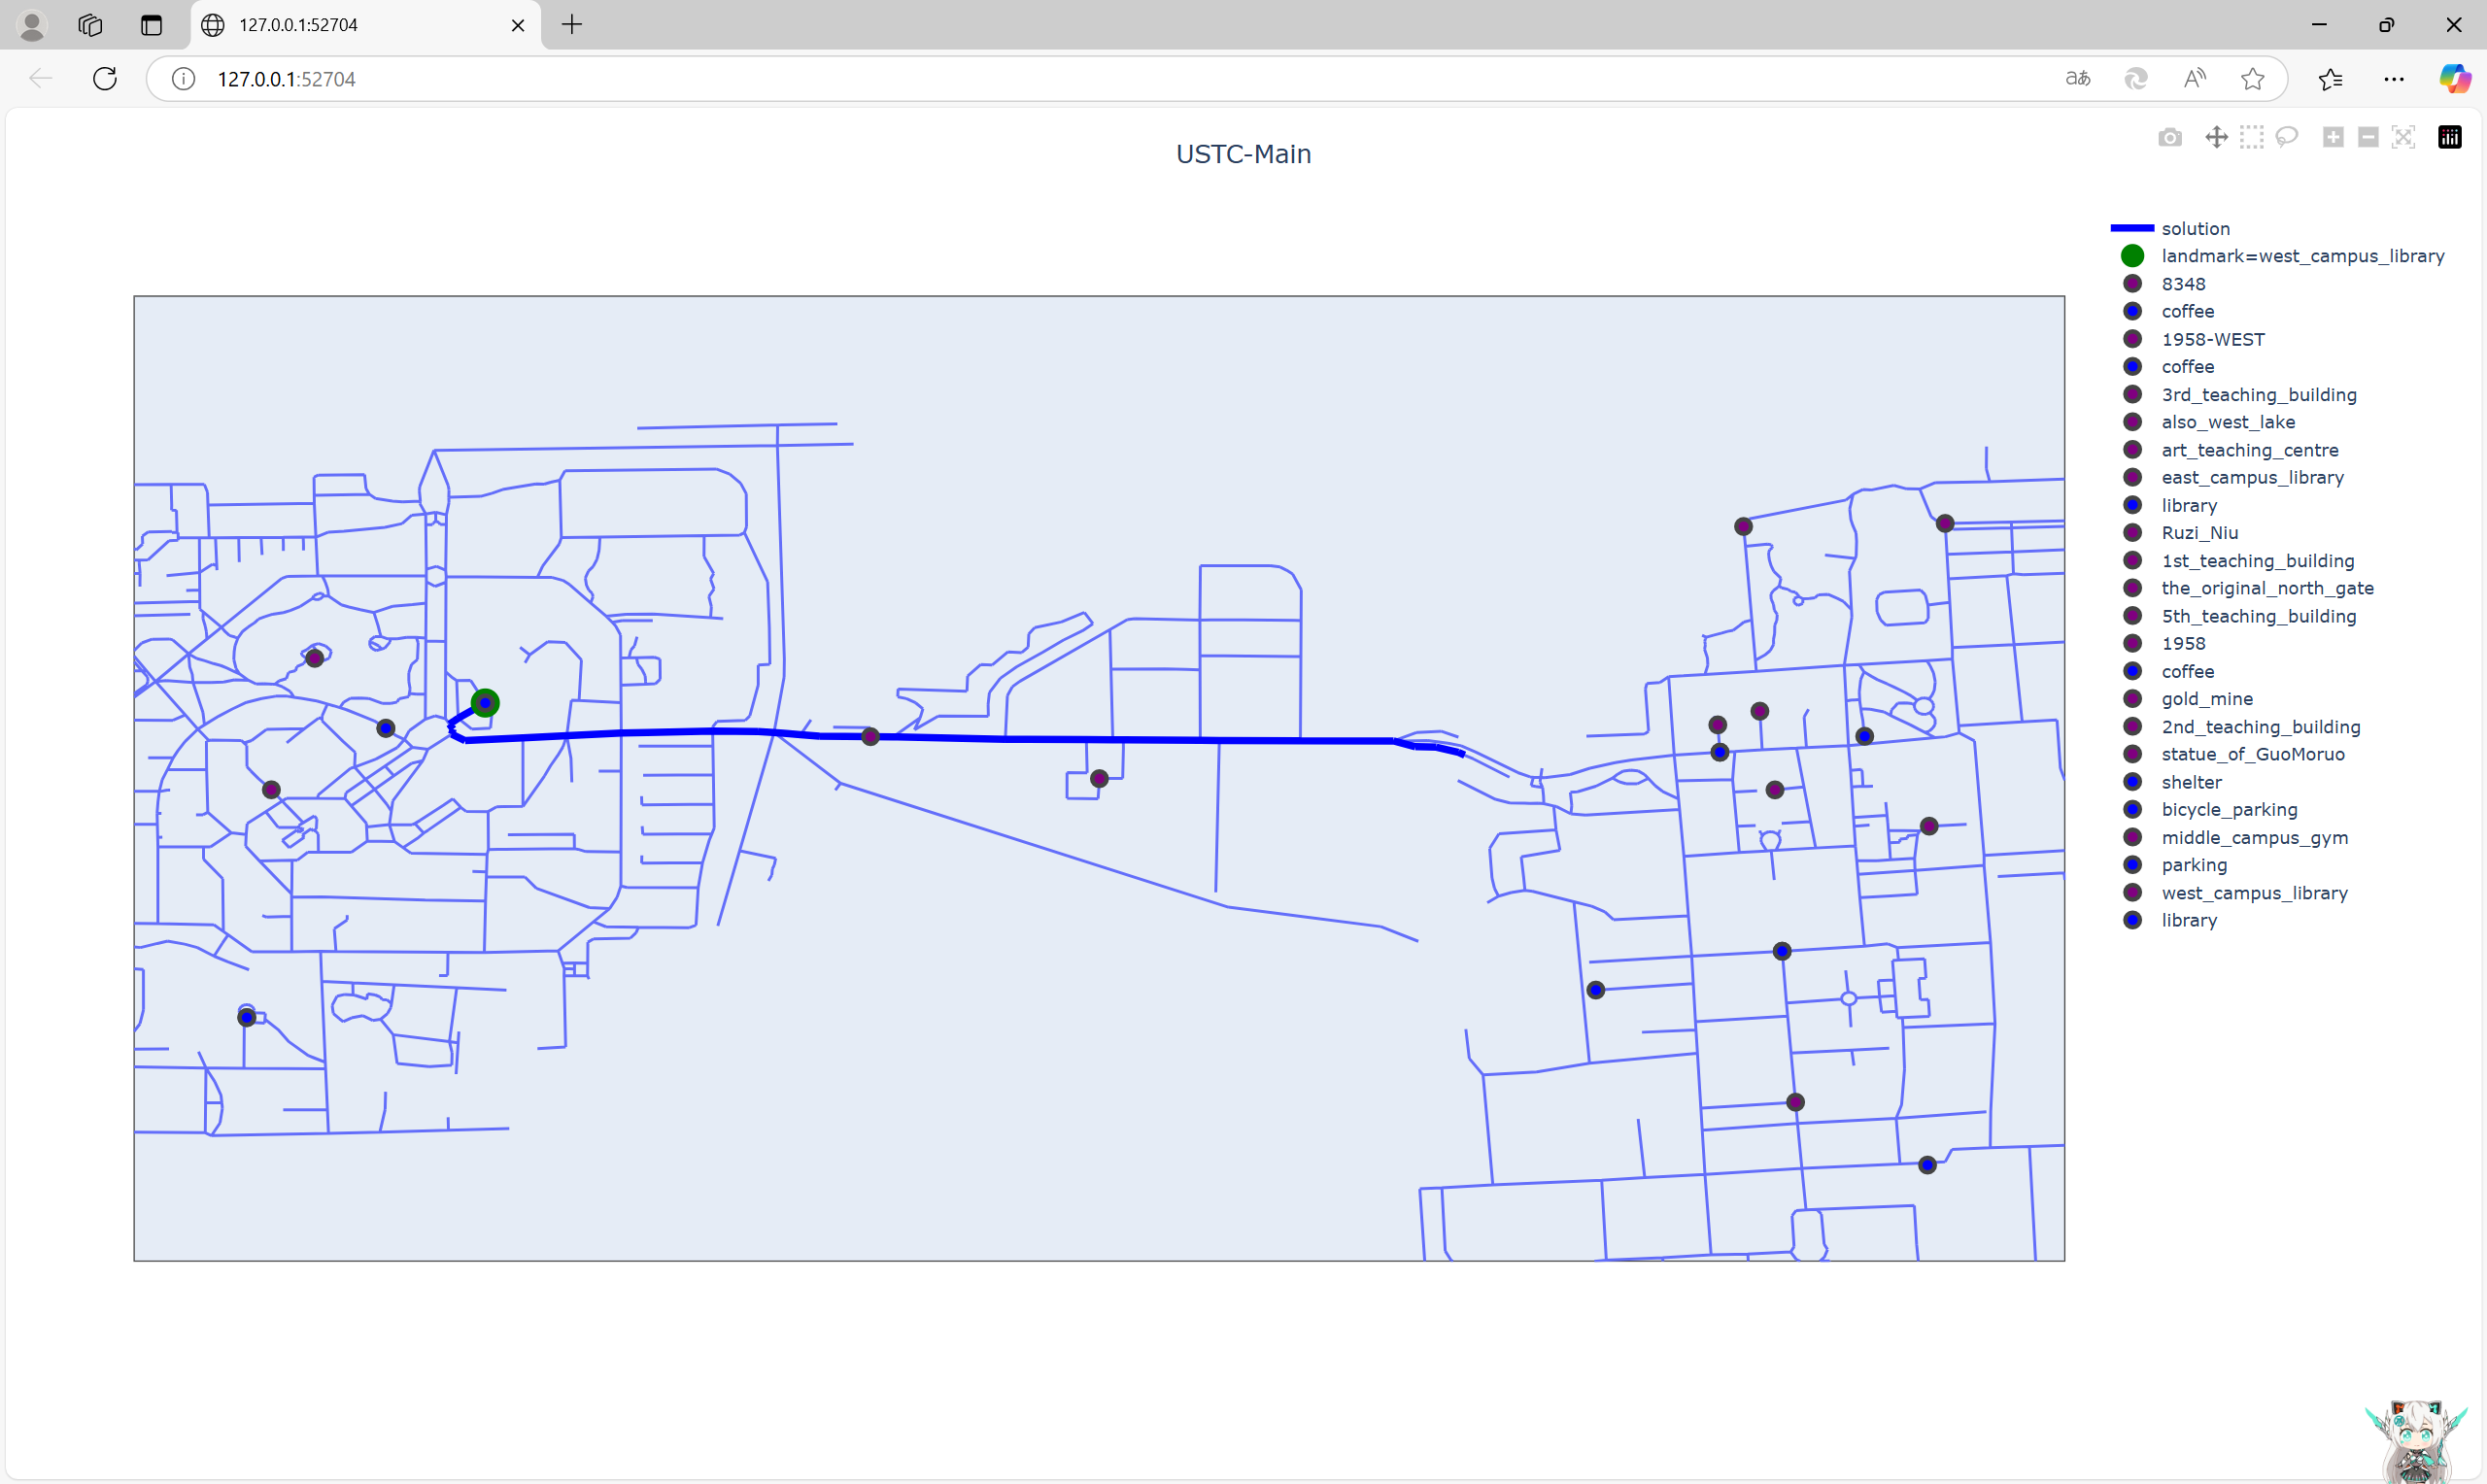
\includegraphics[width=0.8\textwidth]{library_to_gate.png}
    	\caption{中区东门到西区图书馆的最短路径}
    \end{figure}
    
    
\end{enumerate}

\subsection{算法[19\%=6\%+5\%+2\%+6\%]}

\begin{enumerate}[label=(\alph*), start=3]
    \item \textbf{[简答]} %1c
    根据定义,初始状态为:
    \[
    d_s^{(0)}(u) =
    \begin{cases}
    	0, & \text{若 } u = s, \\
    	+\infty, & \text{否则}.
    \end{cases}
    \]
    显然,\( d_s(u) \leq d_s^{(0)}(u) \) 成立。
    
    根据 Dijkstra 算法的递推公式:
    \[
    d_s^{(k+1)}(u) = \min_{v \in \{v_0, \dots, v_k\}} \{ d_s^{(k)}(v) + w_{vu} \}.
    \]
    由于 \( d_s^{(k+1)}(u) \) 是从 \( d_s^{(k)}(u) \) 的基础上通过取最小值更新得到的,因此有:
    \[
    d_s^{(k+1)}(u) \leq d_s^{(k)}(u).
    \]
    
    根据最短路径的定义,\( d_s(u) \) 是从源点 \( s \) 到 \( u \) 的最短路径长度,而 \( d_s^{(k)}(u) \) 是第 \( k \) 次迭代时的估计值。由于 \( d_s^{(k)}(u) \) 是对 \( d_s(u) \) 的逐步逼近,因此有:
    \[
    d_s(u) \leq d_s^{(k+1)}(u).
    \]
    
    综上所述,得到:
    \[
    d_s(u) \leq d_s^{(k+1)}(u) \leq d_s^{(k)}(u).
    \]
    \item \textbf{[简答]} %1d
    假设在第 \( k \) 次迭代中,已经有:
    \[
    d_s^{(k)}(v_k) = d_s(v_k),
    \]
    即当前选中的节点 \( v_k \) 的最短路径距离已经被正确计算。
    
    当 \( k = 0 \) 时,初始节点 \( v_0 = s \),且 \( d_s^{(0)}(s) = 0 \)。显然:
    \[
    d_s^{(0)}(v_0) = d_s(v_0).
    \]
    
    假设对于第 \( k \) 次迭代,已经有 \( d_s^{(k)}(v_k) = d_s(v_k) \)。在第 \( k+1 \) 次迭代中:
    - 根据 Dijkstra 算法,选择满足:
    \[
    v_{k+1} = \arg\min_{u \in V \setminus \{v_0, \dots, v_k\}} d_s^{(k)}(u).
    \]
    - 由于 \( v_{k+1} \) 是当前未访问节点中估计距离最小的节点,且 \( d_s^{(k)}(v_{k+1}) \) 是通过所有可能路径的最小值计算得到的,因此:
    \[
    d_s^{(k+1)}(v_{k+1}) = d_s(v_{k+1}).
    \]
    
    通过数学归纳法可知,对于任意 \( k \),都有:
    \[
    d_s^{(k)}(v_k) = d_s(v_k).
    \]
    当算法执行 \( n-1 \) 次迭代后,所有节点的最短路径距离均已被正确计算。
    
\end{enumerate}

\begin{enumerate}[label=(\alph*), start=5]
    \item \textbf{[判断]} %1e
    不能
    \item \textbf{[简答]} %1f
    (1)在 (d) 的证明中,我们通过数学归纳法证明了 Dijkstra 算法在每次迭代中,当前选中的节点 $ v_k $ 的最短路径距离 $ d_s(v_k) $ 已经被正确计算。这一结论依赖于以下两个核心假设:
    
    非负边权假设:Dijkstra 算法假设图中所有边的权值 $ w_{uv} \geq 0 $。这是因为算法在每次迭代中选择当前估计距离最小的节点 $ v_k $,并将其标记为已访问(即认为 $ v_k $ 的最短路径已经确定)。如果存在负权边,则可能在访问 $ v_k $ 后,通过负权边更新其他节点的距离,导致之前的选择不再最优。\\
    贪心策略的正确性:由于边权非负,Dijkstra 算法的贪心策略能够保证每次选择的节点 $ v_k $ 的最短路径距离不会被后续更新。\\
    因此,Dijkstra 算法无法直接处理存在负权边的图,因为负权边会破坏上述假设,导致算法无法正确计算最短路径。\\
    (2)为了使程序能够在存在负权边的情况下正确运行,可以使用 Bellman-Ford 算法。Bellman-Ford 算法通过多次松弛操作,逐步逼近最短路径,并能够正确处理负权边。
    \begin{lstlisting}[language=Python]
    def bellman_ford(graph, source):
    	distance = {node: float('inf') for node in graph.nodes}
    	distance[source] = 0
    
    	for _ in range(len(graph.nodes) - 1):
    		for u, v, weight in graph.edges:  
    			if distance[u] + weight < distance[v]:
    				distance[v] = distance[u] + weight
    
    	for u, v, weight in graph.edges:
    		if distance[u] + weight < distance[v]:
    			raise ValueError("Graph contains a negative weight cycle")
    
    	return distance
    
    class ShortestPathProblem(SearchProblem):
    	def solve(self):
    		if all(weight >= 0 for _, _, weight in self.cityMap.edges):
    			return dijkstra(self.cityMap, self.startLocation)
    		else:
    			return bellman_ford(self.cityMap, self.startLocation)
    \end{lstlisting}
\end{enumerate}

\section{问题 2:查找带无序途径点的最短路径[17\%]}

\subsection{建模[10\%=6\%+4\%]}

\begin{enumerate}[label=(\alph*), start=1]

    \item \textbf{[代码]} %2a
    \begin{lstlisting}[language=Python]
    class WaypointsShortestPathProblem(SearchProblem):
    	def __init__(
    		self, startLocation: str, waypointTags: List[str], endTag: str, cityMap: CityMap
    	):
    		self.startLocation = startLocation
    		self.endTag = endTag
    		self.cityMap = cityMap
    		self.waypointTags = tuple(sorted(waypointTags))
    
    	def startState(self) -> State:
    		return State(location=self.startLocation, memory=frozenset(self.waypointTags))
    
    	def isEnd(self, state: State) -> bool:
    		return (
    			not state.memory  # All waypoint tags have been covered
    			and self.endTag in self.cityMap.tags.get(state.location, [])
    		)
    
    	def successorsAndCosts(self, state: State) -> List[Tuple[str, State, float]]:
    		successors = []
    		currentLocation = state.location
    		remainingTags = state.memory
    
    		for neighbor, cost in self.cityMap.distances.get(currentLocation, {}).items():
    			newTags = set(remainingTags)
    			for tag in self.cityMap.tags.get(neighbor, []):
    				if tag in newTags:
    					newTags.remove(tag)
    
    			newState = State(location=neighbor, memory=frozenset(newTags))
    			successors.append((neighbor, newState, cost))
    
    		return successors
    \end{lstlisting}
    \item \textbf{[代码]}\textbf{[截图]} %2b
    \begin{lstlisting}[language=Python]
    def getUSTCWaypointsShortestPathProblem() -> WaypointsShortestPathProblem:
    	cityMap = createUSTCMap()
    	startLocation = "10588133363"
    	waypointTags = ["landmark=8348", "landmark=also_west_lake","landmark=art_teaching_centre"]
    	endTag = "landmark=west_campus_library"
    	return WaypointsShortestPathProblem(startLocation, waypointTags, endTag, cityMap)
    \end{lstlisting}
    \begin{figure}[h]
    	\centering
    	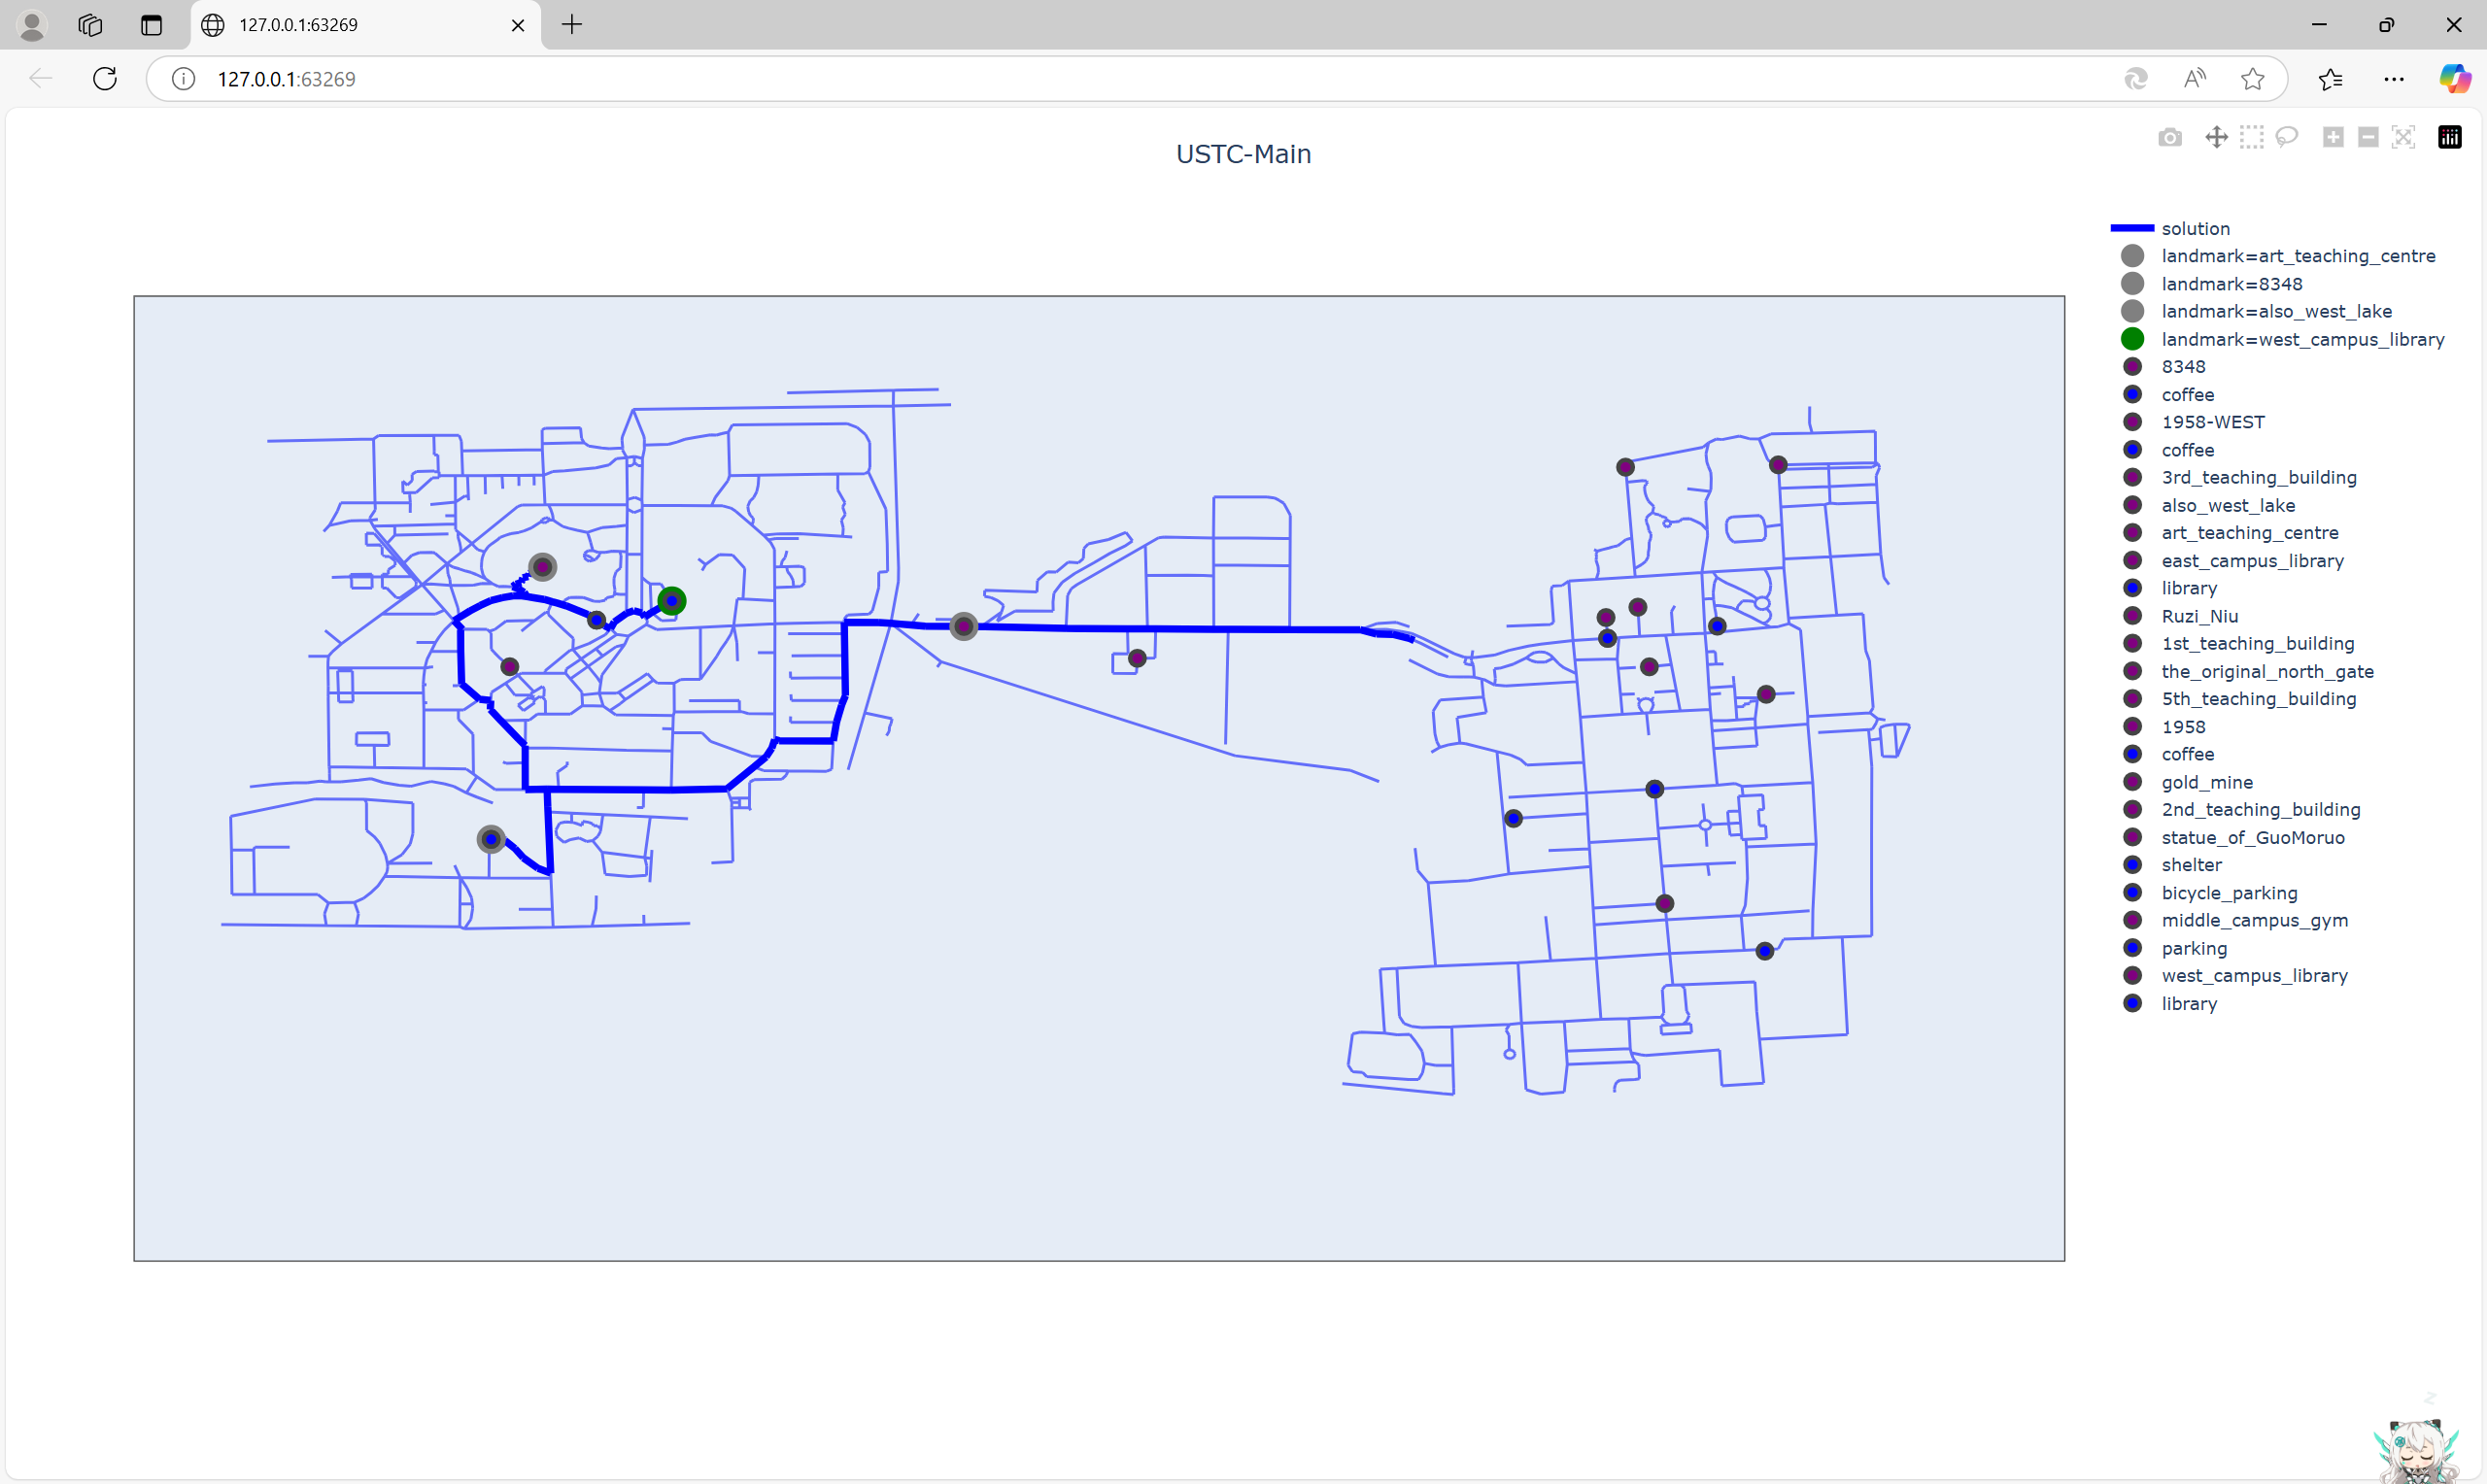
\includegraphics[width=0.8\textwidth]{library_to_gate_waytags.png}
    	\caption{中区东门到西区图书馆,途径8348、也西湖、艺术教学中心的最短路径}
    \end{figure}
\end{enumerate}

\subsection{算法[7\%=2\%+5\%]}

\begin{enumerate}[label=(\alph*), start=3]

    \item \textbf{[判断]} %2c
    不会,将艺术教学中心设为终点,西图、8348、也西湖作为途径点测试结果如下
    \FloatBarrier
    \begin{figure}[h]
    	\centering
    	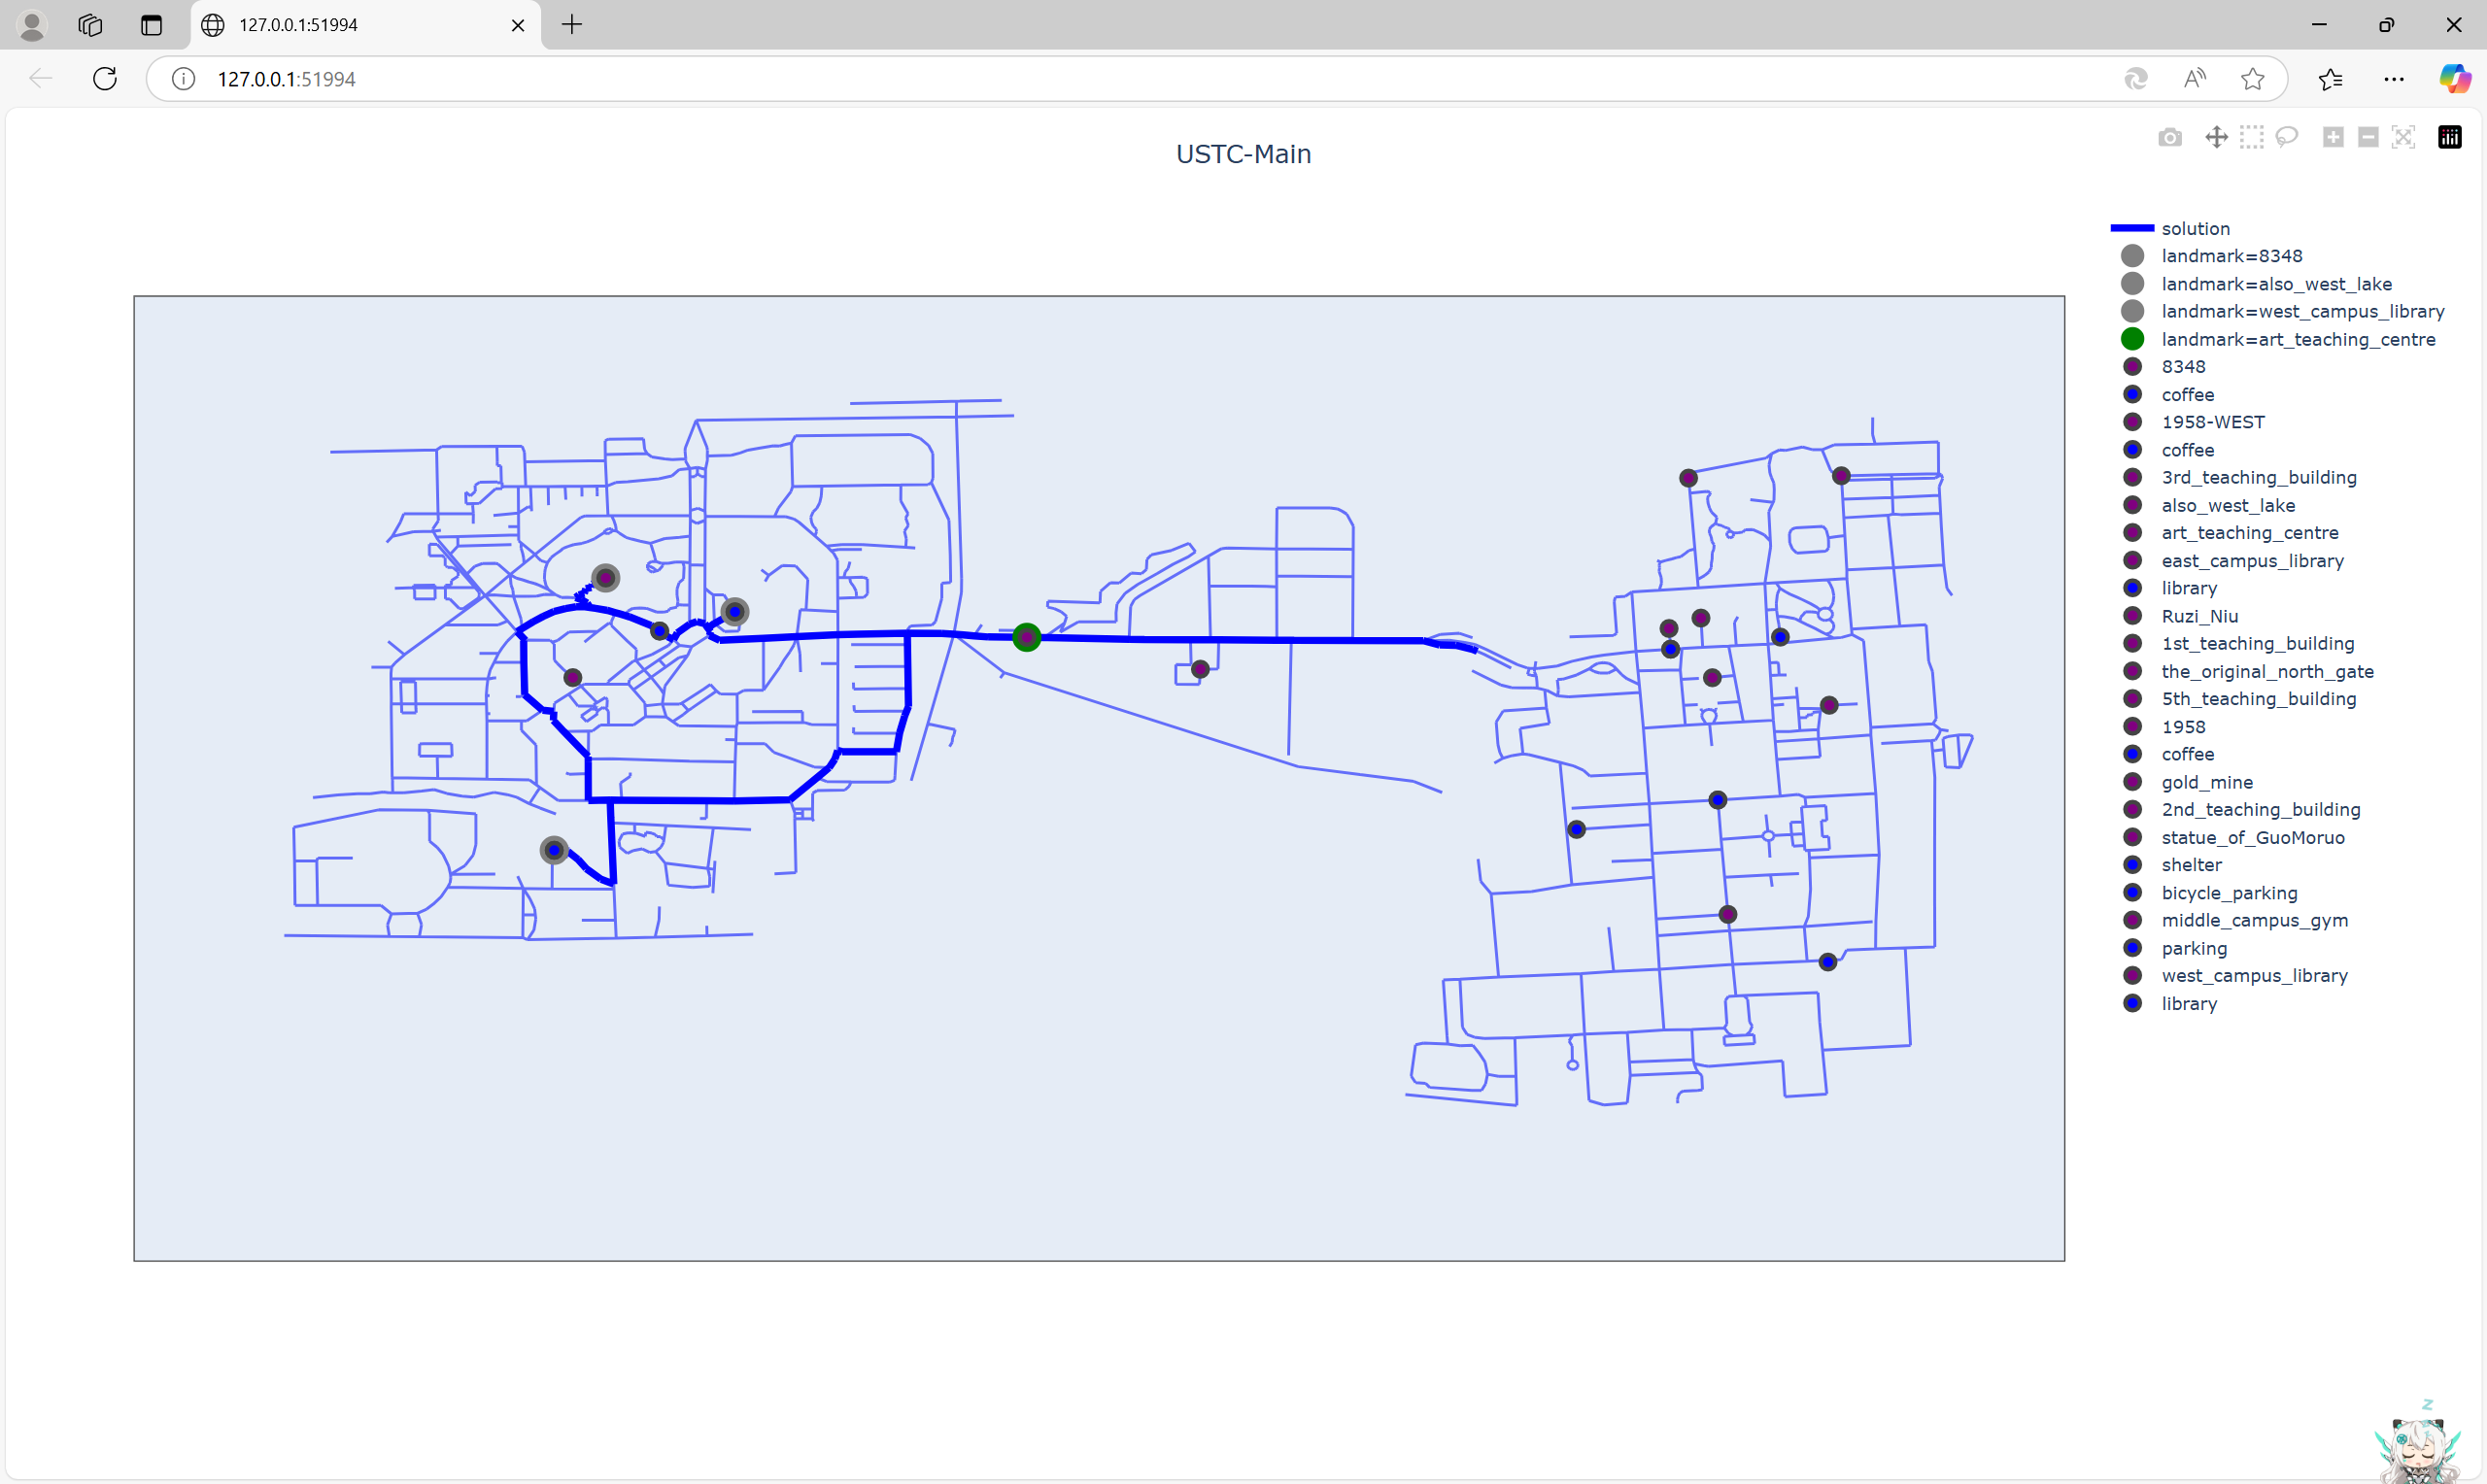
\includegraphics[width=0.8\textwidth]{test_for_duplicate_points.png}
    	\caption{中区东门到艺术教学中心,途径8348、也西湖、西图的最短路径}
    \end{figure}
    \item \textbf{[简答]} %2d
    小李的质疑不成立。带有无序途径点的最短路径问题通过扩展状态定义(包括 \( memory \))和正确的搜索逻辑,能够保证算法的正确性和最优性,不会违反 Dijkstra 算法的性质 \( d_s(u) \leq d_s^{(k)}(u) \)。
    
    1. 在 \texttt{WaypointsShortestPathProblem} 中,状态由 \( (location, memory) \) 表示,其中:\( location \) 是当前所在的位置;\( memory \) 是一个 \texttt{frozenset},表示尚未覆盖的途径点标签集合。
    由于状态包含了 \( memory \),算法在搜索过程中会将路径的代价与尚未覆盖的途径点关联起来。即使路径先到达终点 \( B \),但如果 \( memory \) 中仍有未覆盖的途径点(如 \( X \)),算法会继续探索其他路径以覆盖这些途径点。
    
    2.  Dijkstra 算法的性质 \( d_s(u) \leq d_s^{(k)}(u) \) 是基于以下前提:
    \begin{itemize}
    	\item 每个状态的估计代价是单调递增的;
    	\item 每个状态只会被访问一次。
    \end{itemize}
    
    在 \texttt{WaypointsShortestPathProblem} 中,状态不仅由位置 \( location \) 决定,还包括 \( memory \)。因此,即使两次访问同一个位置 \( B \),但如果 \( memory \) 不同,这两个状态是不同的,且它们的代价是独立计算的。
    
    3. 当路径先到达 \( B \) 而未覆盖所有途径点时:算法会继续探索其他路径,以覆盖 \( memory \) 中的剩余途径点;由于状态包含 \( memory \),算法会记录从 \( B \) 出发覆盖剩余途径点的代价,并将其与之前的路径代价相加;这种回溯行为不会违反 Dijkstra 算法的性质,因为每个状态的代价是独立计算的,且状态的估计代价仍然是单调递增的。
    
    4. 算法最终会找到一条路径,使得:
    \begin{itemize}
    	\item 覆盖所有途径点;
    	\item 到达终点 \( B \);
    	\item 总路径代价最小。
    \end{itemize}
    
    这是因为 Dijkstra 算法的优先队列机制保证了每个状态的代价是按从小到大的顺序处理的,且状态的定义确保了途径点的约束条件被正确处理。
    
    
\end{enumerate}

\section{问题 3:使用 A* 加快搜索速度[32\%]}

\subsection{将UCS转化为A*[4\%]}

\begin{enumerate}[label=(\alph*), start=1]
    \item \textbf{[代码]} %3a
    \begin{lstlisting}[language=Python]
    def aStarReduction(problem: SearchProblem, heuristic: Heuristic) -> SearchProblem:
    	class NewSearchProblem(SearchProblem):
    		def __init__(self):
    			self.problem = problem
    			self.heuristic = heuristic
    
    		@property
    		def startLocation(self) -> str:
    			return self.problem.startLocation
    
    		@property
    		def endTag(self) -> str:
    			return self.problem.endTag
    
    		def startState(self) -> State:
    			return self.problem.startState()
    
    		def isEnd(self, state: State) -> bool:
    			return self.problem.isEnd(state)
    
    		def successorsAndCosts(self, state: State) -> List[Tuple[str, State, float]]:
    			successors = []
    			current_h = self.heuristic.evaluate(state)
    			for action, newState, cost in self.problem.successorsAndCosts(state):
    				new_cost = cost + self.heuristic.evaluate(newState) - current_h
    				successors.append((action, newState, new_cost))
    			return successors
    
    	return NewSearchProblem()
    \end{lstlisting}
\end{enumerate}

\subsection{实现启发式函数[18\%=3\%+6\%+3\%+6\%]}

\begin{enumerate}[label=(\alph*), start=2]
    \item \textbf{[简答]} %3b
    假设对于任意状态(结点) $u$ 和其相邻结点 $v$(即存在一条边 $(u,v)$ 且代价为 $c(u,v)$),直线距离启发式函数定义为
    \[
    h(u) = \text{直线距离}(u, t),
    \]
    其中 $t$ 是终点。根据欧几里得空间中的三角不等式,有
    \[
    \text{直线距离}(u,t) \leq \text{直线距离}(u,v) + \text{直线距离}(v,t).
    \]
    由于实际边的代价 $c(u,v)$ 总是不小于结点 $u$ 和 $v$ 的直线距离(即我们假定地图中边的代价是距离的一种衡量指标,而直线距离作为下界),因此有
    \[
    \text{直线距离}(u,v) \leq c(u,v).
    \]
    将上述两个不等式合并,可得
    \[
    h(u) = \text{直线距离}(u,t) \leq c(u,v) + \text{直线距离}(v,t) = c(u,v) + h(v).
    \]
    这正是启发式函数一致性要求,即对于所有相邻的 $u$ 和 $v$ 有
    \[
    h(u) \leq c(u,v) + h(v).
    \]
    
    因此,使用每个结点到终点的直线距离作为启发式函数满足一致性条件。一致性确保了 A* 算法中每次扩展时 $f$ 值($f(u)=g(u)+h(u)$)是非递减的,从而保证了算法的正确性和最优性。
    
    \item \textbf{[代码]} %3c
    \begin{lstlisting}[language=Python]
    class StraightLineHeuristic(Heuristic):
    	def __init__(self, endTag: str, cityMap: CityMap):
    		self.endTag = endTag
    		self.cityMap = cityMap
    
    	endLocation = locationFromTag(endTag, cityMap)
    	if endLocation is None:
    		raise ValueError("No location with the specified endTag found in cityMap.")
    	self.endLocation = endLocation
    	self.endGeo = cityMap.geoLocations[endLocation]
    
    	def evaluate(self, state: State) -> float:
    		currentGeo = self.cityMap.geoLocations[state.location]
    		return computeDistance(currentGeo, self.endGeo)
    \end{lstlisting}
\end{enumerate}

对于问题2,我们使用不带途径点的最短路径长度作为启发式函数。

\begin{enumerate}[label=(\alph*), start=4]
    \item \textbf{[简答]} %3d
    我们定义启发式函数
    \[
    h(u) = \text{从节点 } u \text{ 到目标集合中任一目标的最短路径长度},
    \]
    其中该最短路径是在忽略所有途径点约束的图上计算得到的。设对于任意相邻节点 $u$ 和 $v$(即存在边 $(u,v)$ 且其代价为 $c(u,v)$),令目标为 $t$,并假设从 $u$ 到 $t$ 的最短路径经过 $v$ 的最短路径是最优的,则有
    \[
    h(u) = \text{cost}(u,t) \leq c(u,v) + \text{cost}(v,t) = c(u,v) + h(v).
    \]
    这里的不等式成立,其原因是最短路径满足三角不等式:从 $u$ 到 $t$ 的最短距离不可能超过经过 $v$ 再到 $t$ 的距离。
    
    因此,对于任意相邻节点 $u$ 和 $v$ 都有
    \[
    h(u) \leq c(u,v) + h(v),
    \]
    这正是启发式函数一致性的定义。由此可知,使用不带途径点的最短路径长度作为启发式函数是\textbf{一致}的。
    
    一致性保证了在 A* 算法中,每次扩展时节点的 $f$ 值(即 $f(u) = g(u) + h(u)$)不会出现下降,从而确保了算法能够以正确顺序展开搜索并找到最优解。
    
    \item \textbf{[代码]} %3e
    \begin{lstlisting}[language=Python]
    class NoWaypointsHeuristic(Heuristic):
    	def __init__(self, endTag: str, cityMap: CityMap):
    		self.endTag = endTag
    		self.cityMap = cityMap
    		self.targetLocations = []
    		for loc, tags in cityMap.tags.items():
    			if endTag in tags:
    				self.targetLocations.append(loc)
    		if not self.targetLocations:
    			raise ValueError("No location with the specified endTag found in cityMap.")
    		self.distanceToGoal = {}  
    		pq = []  
    		for target in self.targetLocations:
    			self.distanceToGoal[target] = 0.0
    			heapq.heappush(pq, (0.0, target))
    		while pq:
    			d, loc = heapq.heappop(pq)
    			if d > self.distanceToGoal.get(loc, float('inf')):
    				continue
    			for neighbor, cost in cityMap.distances.get(loc, {}).items():
    				newd = d + cost
    				if newd < self.distanceToGoal.get(neighbor, float('inf')):
    					self.distanceToGoal[neighbor] = newd
    					heapq.heappush(pq, (newd, neighbor))
    
    	def evaluate(self, state: State) -> float:
    		return self.distanceToGoal.get(state.location, float('inf'))
    \end{lstlisting}
\end{enumerate}

\subsection{利用合肥市地图对比运行时间[10\%=4\%+6\%]}

\begin{enumerate}[label=(\alph*), start=6]
    \item \textbf{[代码]}{[简答]} %3f
    \begin{lstlisting}[language=Python]
    def getHefeiShortestPathProblem(cityMap: CityMap) -> ShortestPathProblem:
    	startLocation=locationFromTag(makeTag("landmark", "USTC"), cityMap)
    	endTag=makeTag("landmark", "Chaohu")
    	return ShortestPathProblem(startLocation, endTag, cityMap)
    
    def getHefeiShortestPathProblem_withHeuristic(cityMap: CityMap) -> ShortestPathProblem:
    	startLocation=locationFromTag(makeTag("landmark", "USTC"), cityMap)
    	endTag=makeTag("landmark", "Chaohu")
    	baseProblem = ShortestPathProblem(startLocation, endTag, cityMap)
    	heuristic = StraightLineHeuristic(endTag, cityMap)
    	return aStarReduction(baseProblem, heuristic)
    \end{lstlisting}
    运行 python grader.py 3f-without\_Heuristic 和 python grader.py 3f-with\_Heuristic 所需时间分别为1.586795秒和0.716272秒,运行结果如下图
    \FloatBarrier
    \begin{figure}[h]
    	\centering
    	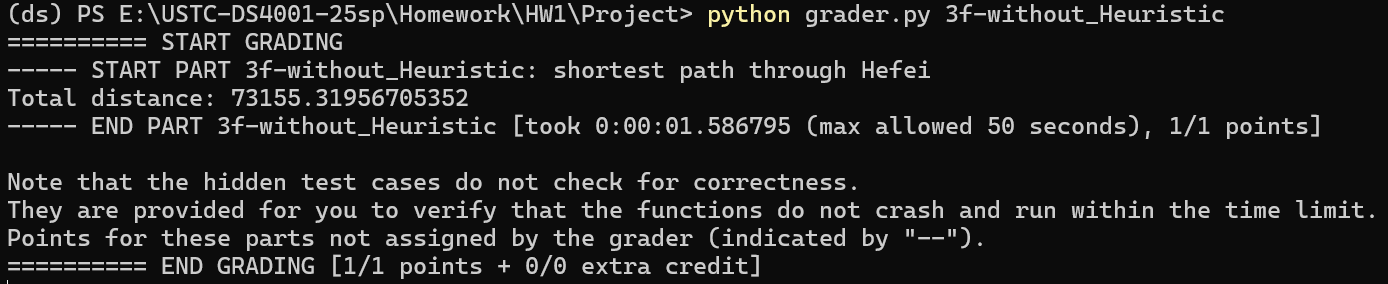
\includegraphics[width=0.8\textwidth]{3f-without_Heuristic.png}
    	\caption{3f-without\_Heuristic}
    	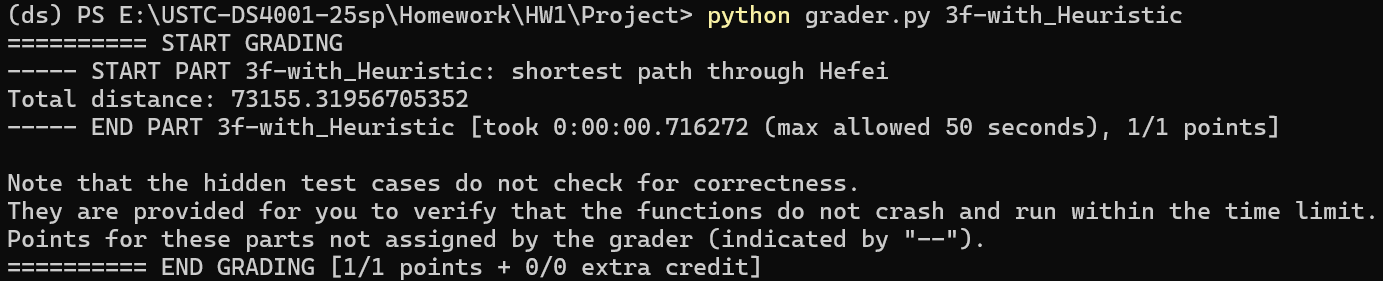
\includegraphics[width=0.8\textwidth]{3f-with_Heuristic.png}
    	\caption{3f-with\_Heuristic}
    \end{figure}
    \FloatBarrier
    \item \textbf{[简答]} %3g
    在合肥市地图上运行时,可能存在以下几个缺陷:
    \begin{enumerate}
    	\item 状态空间大、搜索节点过多:合肥地图规模较大,导致需要扩展的状态数量剧增,即使用了一些启发式重加权方法,也有可能存在许多低质量或冗余的扩展,增加运行时间
    	\item 启发式函数计算效率问题:在每次扩展节点时,程序会反复调用启发式函数(如 StraightLineHeuristic 或 NoWaypointsHeuristic)的 evaluate 方法。虽然这些方法本身很快,但在大图中调用次数可能非常多,整个搜索过程会因此开销较大。
    	\item 重复计算和状态查找:如果状态表示的设计不够高效(例如内存中存储的状态没有进行良好的去重或哈希优化),可能会导致重复计算或多次访问相同结点,从而拖慢搜索速度。
    \end{enumerate}
    为进一步减少运行时间,可以考虑预处理与双向搜索结合的改进方案\\
    主要思路
    \begin{enumerate}
    	\item 预处理启发式信息(多源 Dijkstra 或 ALT 方法)\\
    	利用预处理方法提前对地图中的节点进行计算,获得每个节点到目标(或目标集合)的最短距离估计。这样在搜索过程中,每次调用启发式函数时,只需查表返回对应值,而不必重复计算距离。\\
    	- 例如,对 Hefei 地图可以用多源 Dijkstra 算法预先计算所有节点到目标集合的最短距离,将结果存入一个字典中;在 NoWaypointsHeuristic.evaluate 中直接返回查表结果。如果地图节点非常多,可以采用ALT(A*, Landmarks, and Triangle inequality)算法,该方法利用一组预选地标,提高启发式估计的精确度和计算效率。
    	\item 双向搜索(Bidirectional Search)\\
    	A传统单向搜索在大图中扩展大量节点。利用双向搜索技术,从起点和目标同时开始搜索,并在中间碰撞合并,可以显著减少需要探索的状态数,从而加快搜索速度。\\
    	- 需要注意双向A设计中启发式函数的对称性以及如何实现两侧搜索结果的合并。
    \end{enumerate}\
    详细步骤
    \begin{enumerate}
    	\item 预处理启发式值\\
    	- 在程序启动阶段,对 Hefei 地图使用多源 Dijkstra 算法,计算目标集合(例如 endTag 对应的所有目标)的最短路径距离,并存储结果为字典。\\
    	- 修改启发式类(如 NoWaypointsHeuristic 或 StraightLineHeuristic)的 evaluate 方法,使得其直接从预处理表中返回结果,这样可以减少每次调用 computeDistance 的开销。
    	\item 改进状态数据结构和开放列表管理\\
    	- 保持状态的唯一性,并利用更高效的数据结构(比如更快的哈希表或者 Fibonacci 堆)管理 open list,以降低每次扩展的时间复杂度。
    	\item 实现双向搜索\\
    	- 将搜索算法修改为双向搜索,一端从起点开始,一端从目标出发。两个方向各自运行A*(或经预处理的启发函数支持的A*),当两端的搜索相遇,合并路径并计算总代价。\\
    	- 双向搜索需要设计适合的状态匹配机制和边界条件判断,确保满足最短路径收敛性和正确性。
    \end{enumerate}
    
    
    
    
    
    
    
    
\end{enumerate}

\section*{体验反馈[2\%]}

\begin{enumerate}[label=(\alph*), start=1]
    \item \textbf{[必做]} %所花时间
    大约10h
    \item \textbf{[选做]} %其他反馈
    没有
\end{enumerate}


\end{document}
